\chapter{CAM3 and AM2 cloud response to warming}
\label{cmip3hot}
\section{Introduction}
The simulated climate response to increases in carbon dioxide is known to differ among different climate models. For the past two decades, cloud feedback processes have been recognized as being among the largest sources of inter-model spread in equilibrium climate sensitivity and in uncertainty in future projections of the earth climate system made by climate models \citep{cess_et_al_1990,cess_et_al_1996,colman_2003,soden_and_held_2006,webb_et_al_2006,ar4_ch8}. \cite{stephens_2005} argues that much of the uncertainty in cloud feedbacks in climate models stems from the difficulty in representing cloud processes in model simulations, due to the discrepancy in resolution between that which is practical for global-scale climate models and that which is important for cloud-related processes. The result is that these processes must be parameterized to approximate their effects at the relatively coarse resolution of climate models. \cite{randall_et_al_2003} describe this so-called parameterization problem as an attempt to represent the small-scale effects, such as clouds, in terms of the large-scale system. This is a difficult process as the connection between effects at the two scales is not constrained by a single physical theory, and different modelers may take different approaches to the problem. The high level of empiricism and differences in approach to this problem leads to high levels of uncertainty in the representation of clouds in climate models and especially in the simulated responses of clouds to climate change. Numerous studies have demonstrated that the sensitivity of climate models depends on the representation of clouds \citep[e.g.,][]{mitchell_et_al_1987,senior_and_mitchell_1993,le_treut_et_al_1994,fowler_and_randall_1994,ma_et_al_1994,liang_and_wang_1997,yao_and_del_genio_2002,zhang_2004,stainforth_et_al_2005,yokohata_et_al_2005}, and \cite{stephens_2005} emphasizes the critical importance of progress on the cloud parameterization problem to the progress of the cloud feedback problem. 

Evaluations of model simulated clouds for present day climate simulations are an important first step toward assessing the representation of clouds in climate models. Evaluating the response of climate model simulations to climate change scenarios is nontrivial, as observational data is not available for comparison. This leaves open the question of how clouds can be expected to respond to a changing climate, and numerous hypotheses have been suggested.

The tropics are characterized by large over-turning circulations, giving rise to regions of deep convection and associated anvil-forming clouds, and regions of subsidence and associated boundary layer clouds. How such convective anvil clouds should respond to climate change has been the subject of a number of studies and hypotheses. The ``Fixed-Anvil Temperature'' (FAT) hypothesis of \cite{hartmann_and_larson_2002} suggests that the temperature of the tops of these anvil clouds is essentially independent of the surface temperature, and that their temperature can be expected to remain nearly constant even as surface temperatures rise. The heights of the anvil cloud tops rise in order to stay at the same temperature. This mechanism implies a positive feedback, as the temperature difference between high-topped clouds and the surface increases in a warming climate, leading to an enhanced longwave heating effect. Evidence supporting the fixed-anvil temperature hypothesis has been demonstrated in cloud resolving models \citep{kuang_and_hartmann_2007}, and more recently in climate models \citep{zelinka_and_hartmann_2010}.

There is considerable disagreement on the likely response of the amount of anvil cloud fraction to climate change \citep{ar4_ch8}. The so-called ``iris'' hypothesis \citep{lindzen_et_al_2001} suggests that anvil cloud amount would decrease in response to increasing sea surface temperatures and cause a negative feedback, but this hypothesis has met much criticism \citep{chambers_et_al_2002,del_genio_and_kovari_2002,fu_et_al_2002,harrison_2002,hartmann_and_michelsen_2002,lin_et_al_2002,lin_et_al_2004}.

The response of boundary layer clouds to climate change is not yet well understood \citep{ar4_ch8}. An observed correlation between low-level cloud amount and lower tropospheric stability \citep{klein_and_hartmann_1993} has inspired studies suggesting that low-level cloud amount should increase with increasing sea surface temperature, providing a negative feedback by increasing the shortwave cooling effect of clouds \citep{miller_1997,zhang_2004}, although these results are uncertain. Observational studies have suggested that optical thickness decreases in regions covered by low-level clouds with increasing temperatures, decreasing the shortwave cooling effect of clouds \citep{tselioudis_and_rossow_1994,greenwald_et_al_1995,bony_et_al_1997,del_genio_and_wolf_2000,bony_and_dufresne_2005}. In a warming climate, this would provide a positive feedback, although \cite{ar4_ch8} note again that understanding of this is limited.

\section{Model and experiment set-up}
A simple experiment design to analyze feedbacks was proposed by \cite{cess_and_potter_1988}. It uses a uniform sea surface temperature perturbation as a surrogate for climate change. In this design, the climate change is essentially prescribed, and the response of the system to the prescribed change can be studied. This concept has been used in a number of studies to study feedbacks \cite[e.g.,][]{cess_et_al_1990,cess_et_al_1996}, but others have pointed to differences in feedbacks calculated using the methods of \cite{cess_and_potter_1988} and traditional full feedback calculations using coupled models \citep{senior_and_mitchell_1993,soden_et_al_2004,ringer_et_al_2006}. More recently, \cite{gettelman_et_al_2011} looked at feedbacks in two recent versions of the NCAR CAM using a similar experiment design, but replacing the uniform sea surface temperature perturbation with a spatially varying perturbation determined from a slab ocean model climate change simulation.

Despite the limitations of the method proposed by \cite{cess_and_potter_1988} for diagnosing feedbacks, the concept of using a sea surface temperature perturbation as a surrogate for climate change has proven to be quite useful. This concept is used here to assess the changes in clouds in response to a prescribed climate change in the two models evaluated in Chapter \ref{cmip3amip}. Each model is forced with the same observed, monthly-evolving sea surface temperatures used in the AMIP simulations, but with a uniform $+4~\text{K}$ temperature perturbation applied. A $+4~\text{K}$ perturbation was used rather than the typical $\pm 2~\text{K}$ perturbation used in previous feedback studies in order to increase the signal using only a single simulation. These ``HOT4K'' simulations were run for the ten-year period from 1990-1999, with a one-year spin-up started in 1989 not included in the reported climatologies.

The response of the clouds in the perturbed sea surface temperature simulations are assessed using satellite instrument simulators. The benefit of using satellite instrument simulators in this case is not to facilitate comparisons between model and observations, as observations are not available for the perturbed climate. Rather, the simulator approach allows comparisons of radiatively important cloud statistics between the control and perturbed model climates, as well as providing a common framework in which to compare the responses of the two models. In addition, this approach gives at least an estimate of how the real-world clouds might be expected to respond as seen by the available instruments in a similarly perturbed climate, and gives some insight into the ability of these instruments to detect changes in the clouds brought about by climate change.

\section{Results}
The NCAR CAM3 and GFDL AM2 are chosen for this study in large part because of their known differing responses to climate change (e.g. \cite{stephens_2005}, Figure 1, although this is an earlier version of the CAM than used here). This is immediately apparent in Figures \ref{swcrechanges_cmip3hot4k_map} and \ref{lwcrechanges_cmip3hot4k_map}, which show the changes in the shortwave and longwave cloud radiative effect between the AMIP and HOT4K simulations. The changes in both the regional and globally averaged shortwave and longwave cloud radiative effect terms are quite different between the two models. The CAM3 simulation shows an increase in the magnitude of both the global annual mean shortwave and longwave cloud radiative effect, while the AM2 simulation shows no appreciable change in the global annual mean. 

The differences in the regional responses of the two models are more dramatic. The CAM3 simulation shows an enhancement of both the shortwave and longwave cloud radiative effect through much of the tropical Pacific Ocean and into the southern hemisphere trade cumulus. In contrast, the AM2 simulation shows a weakening of the magnitude of the shortwave cloud radiative effect throughout the subtropical stratocumulus and trade cumulus regions, with an increase in magnitude of the shortwave cloud radiative effect along the ITCZ and in the tropical warm pool.

\begin{figure}
    \centering
    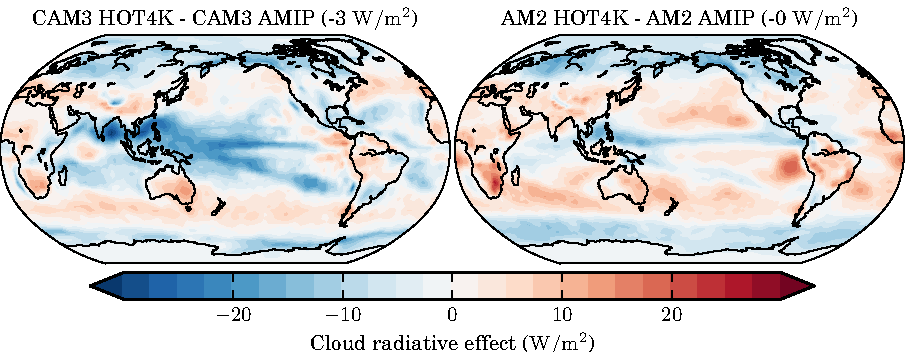
\includegraphics{../graphics/swcrechanges_cmip3hot4k_map.pdf}
    \caption{Changes in shortwave cloud radiative effect between AMIP and HOT4K simulations from CAM3 and AM2.}
    \label{swcrechanges_cmip3hot4k_map}
\end{figure}

\begin{figure}
    \centering
    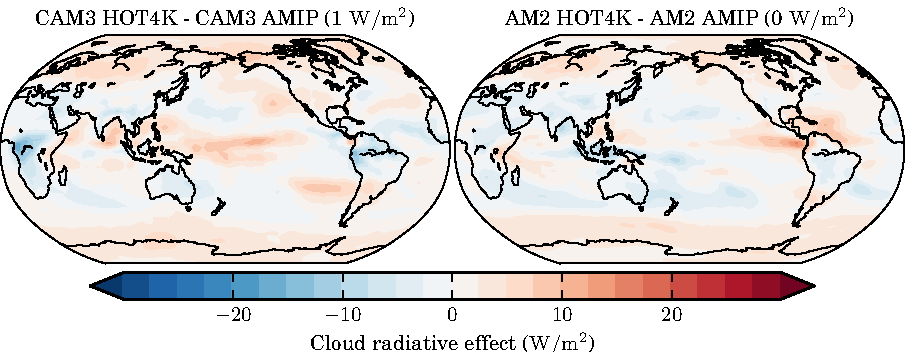
\includegraphics{../graphics/lwcrechanges_cmip3hot4k_map.pdf}
    \caption{Changes in longwave cloud radiative effect between AMIP and HOT4K simulations from CAM3 and AM2.}
    \label{lwcrechanges_cmip3hot4k_map}
\end{figure}


The decrease in magnitude of the shortwave cloud radiative effect in the subtropical marine stratocumulus regions in the AM2 simulation is explained by Figure \ref{hist2d_cmip3hot4k_california}, which shows that low-topped cloud in the California stratocumulus region decreases in the perturbed climate relative to the AMIP simulation. The largest change in cloudiness occurs for low-topped optically intermediate cloud, and in the bins with the highest frequency of occurrence in the AMIP simulation (Figure \ref{hist2d_cmip3amip_california}). In contrast the CAM3 perturbed sea surface temperature simulation shows much less change in low-topped cloud in this region summed across all optical thickness bins, but the distribution with optical thickness has changed, as shown by the increase in low-topped optically thick cloud and the decrease in low-topped optically intermediate cloud. This loosely follows the pattern of the bias in the simulation of the present day climate, which shows a bias toward cloud with higher optical thickness than observed by any of the three instruments considered.

\begin{figure}
    \centering
    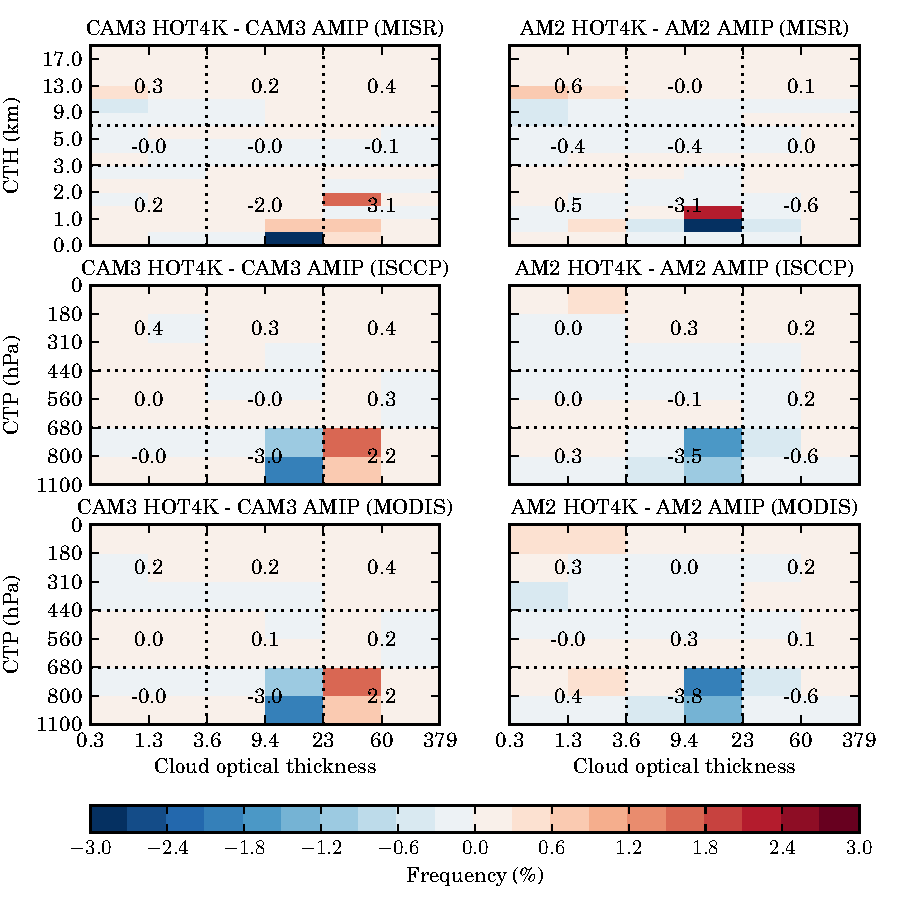
\includegraphics{../graphics/hist2d_cmip3hot4k_california.pdf}
    \caption[California stratocumulus changes in summertime cloudiness with cloud top height and optical thickness between AMIP and HOT4K simulations from CAM3 and AM2.]{California stratocumulus (Table \ref{regions}) changes in summertime (June, July, August) cloudiness with cloud top height and optical thickness between AMIP and HOT4K simulations from CAM3 and AM2.}
    \label{hist2d_cmip3hot4k_california}
\end{figure}

The decrease in the magnitude of the shortwave cloud radiative effect in the Hawaiian trade cumulus in the AM2 simulation is consistent with an overall decrease in cloud amount in this region, especially in high-topped optically thin and low-topped optically intermediate cloud types (Figure \ref{hist2d_cmip3hot4k_hawaiian}). As in the California stratocumulus, the cloud types that change the most are those that have the highest frequency of occurrence in the AMIP simulation, and also represent the cloud types with large biases relative to the observations in the AMIP simulation. The response of the CAM3 simulation again differs from the response of the AM2 simulation. High-topped optically thin cloud decreases similarly, but this is largely compensated for in the CAM3 simulation by an increase in high-topped optically thick cloud, with the net result being much less change in high-topped cloud than seen in the AM2 simulation. The response of the low-topped cloud is quite different in the CAM3 simulation, with a large increase in low-topped cloud mainly due to an increase in low-topped optically thick cloud. Again, the cloud types with the largest changes in the perturbed sea surface temperature simulation seem to be those that occur with large frequency in the AMIP simulations.

\begin{figure}
    \centering
    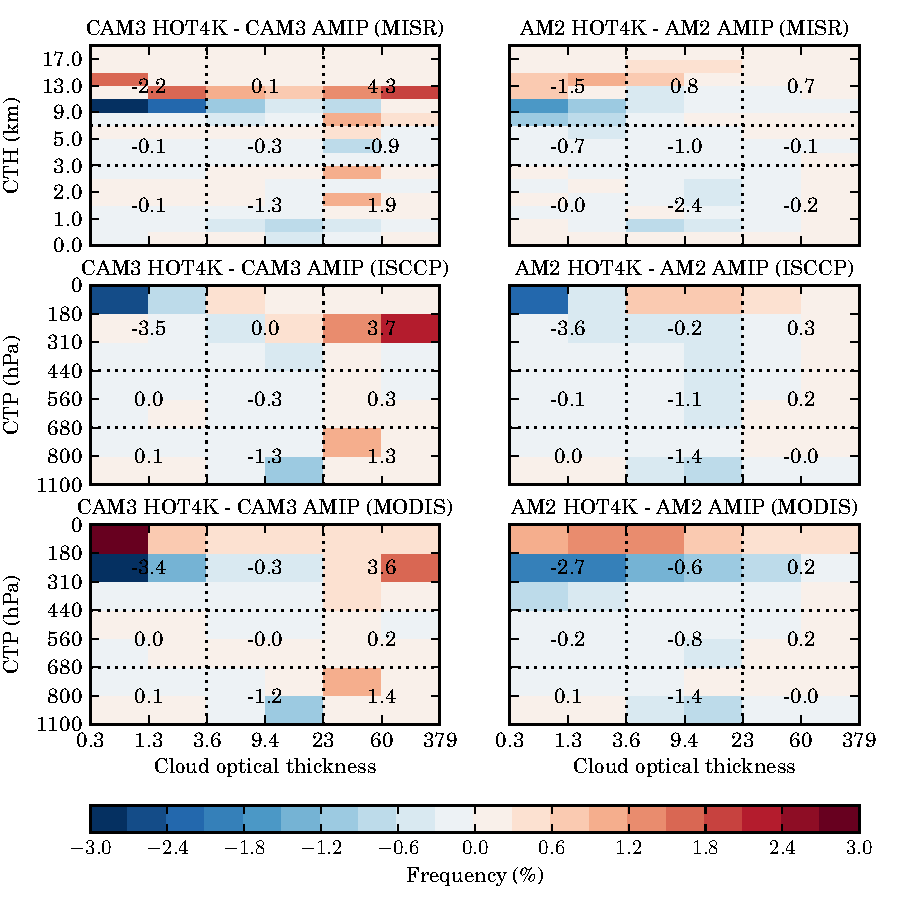
\includegraphics{../graphics/hist2d_cmip3hot4k_hawaiian.pdf}
    \caption[Hawaiian trade cumulus changes in summertime cloudiness with cloud top height and optical thickness between AMIP and HOT4K simulations from CAM3 and AM2.]{Hawaiian trade cumulus (Table \ref{regions}) changes in summertime (June, July, August) cloudiness with cloud top height and optical thickness between AMIP and HOT4K simulations from CAM3 and AM2.}
    \label{hist2d_cmip3hot4k_hawaiian}
\end{figure}

In the deep tropics, both CAM3 and AM2 simulations show increases in the magnitude of both the shortwave and longwave cloud radiative effect, although the increase is much more substantial and widespread in the CAM3 simulation (Figures \ref{swcrechanges_cmip3hot4k_map} and \ref{lwcrechanges_cmip3hot4k_map}). These changes are due to large changes in the high-topped clouds in this region, as shown for the tropical western Pacific in Figure \ref{hist2d_cmip3hot4k_twp}. The increase in the shortwave cloud radiative effect in both CAM3 and AM2 simulations in this region is likely due to the large increases in high-topped optically thick cloud. High-topped optically thick cloud increases more in the CAM3 simulation, causing the larger increase in the shortwave cloud radiative effect seen in Figure \ref{swcrechanges_cmip3hot4k_map}. The increase in high-topped optically thick cloud is partially compensated for in both model simulations by a decrease in high-topped optically thin cloud. In the CAM3 simulation, the increase in high-topped optically thick cloud is greater in magnitude than the decrease in high-topped optically thin cloud, easily explaining the large increase in the magnitude of the longwave cloud radiative effect in this region. The increase in high-topped optically thick and decrease in high-topped optically thin clouds are much closer in magnitude in the AM2 simulation and, in fact, the MODIS simulated cloud actually shows an overall decrease in high-topped cloud. The increase in longwave cloud radiative effect is instead accounted for by an increase in cloud top heights of high-topped cloud in this region. This is clearly demonstrated in the MISR and MODIS-simulated joint histograms of change of cloudiness with cloud top height and optical thickness (upper and lower-right panels of Figure \ref{hist2d_cmip3hot4k_twp}), which show an increase in frequency of high-topped clouds in bins directly above bins that show a corresponding decrease in frequency. Evidence for an upward shift in cloud top heights is seen in the CAM3 perturbed sea surface temperature simulation as well. This rise in cloud top heights is consistent with that predicted by the fixed-anvil temperature hypothesis \citep{hartmann_and_larson_2002,zelinka_and_hartmann_2010}.

\begin{figure}
    \centering
    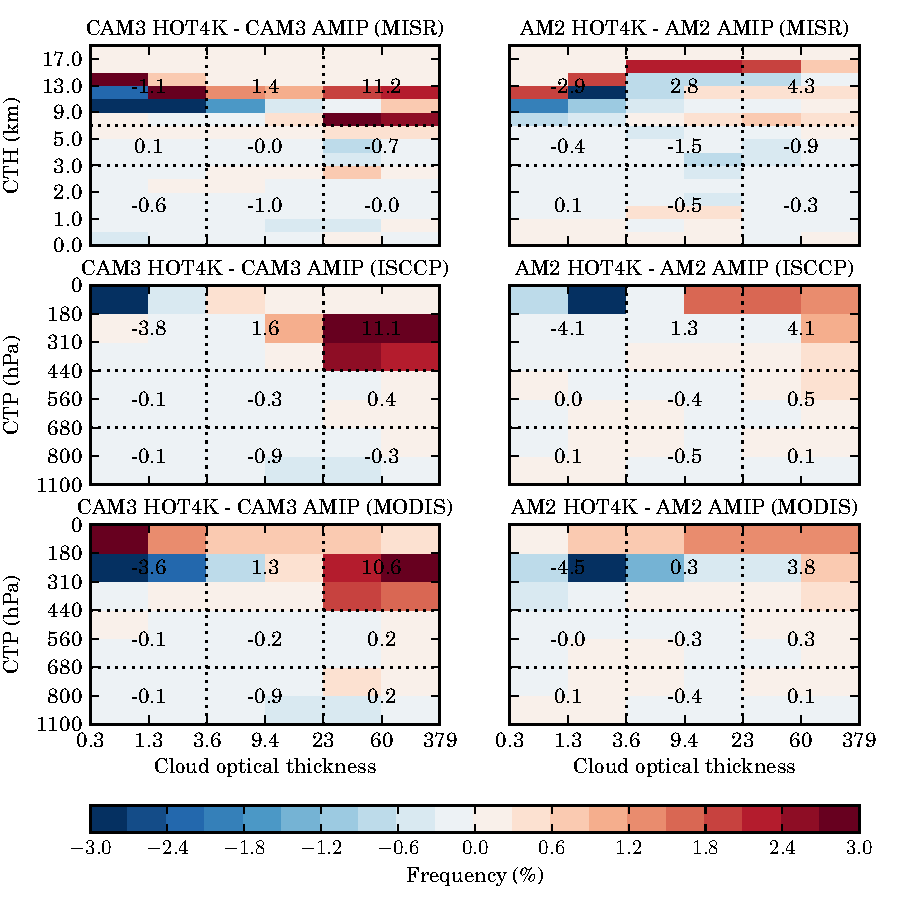
\includegraphics{../graphics/hist2d_cmip3hot4k_twp.pdf}
    \caption[Tropical western Pacific changes in northern hemisphere summertime cloudiness with cloud top height and optical thickness between AMIP and HOT4K simulations from CAM3 and AM2.]{Tropical western Pacific (Table \ref{regions}) changes in northern hemisphere summertime (June, July, August) cloudiness with cloud top height and optical thickness between AMIP and HOT4K simulations from CAM3 and AM2.}
    \label{hist2d_cmip3hot4k_twp}
\end{figure}

\section{Discussion}
The two models considered here have very different cloud responses in regions dominated by boundary layer clouds in the subtropics. Large biases in these cloud types were demonstrated earlier in simulations of present day climate from both models, and their differing responses to increasing sea surface temperatures demonstrated here underscores the concern raised earlier as to the credibility of cloud feedbacks represented by these models. The very differing responses of clouds in these regions is consistent with the implication of \cite{bony_and_dufresne_2005} that the response of these clouds to surface warming are the main source of uncertainty in tropical cloud feedbacks.

Cloud top heights in the deep tropics increase in response to increased sea surface temperatures in both models. This result is consistent with the fixed-anvil temperature hypothesis \citep{hartmann_and_larson_2002}, and explains the increase in the magnitude of longwave cloud radiative effect in the deep tropics in both models. \cite{zelinka_and_hartmann_2010} showed that the cloud top heights of high-topped clouds in the tropics similarly increase in IPCC SRES A2 scenario simulations. The CAM3 simulation also shows a large increase in high-topped optically thick cloud in this region, which is likely to be of greater impact on the longwave cloud radiative effect than the increase of cloud top heights in this region.

Using satellite instrument simulators in the study of the response of clouds to increasing sea surface temperatures provides a common framework for the intercomparison of models, but perhaps more importantly allows for changes in the simulation of the perturbed climate to be assessed in relation to identified biases in the simulation of present day climate. An important result demonstrated here using this technique is that some of the largest changes in the clouds in response to an increase in sea surface temperatures seem to occur in cloud types with have a high frequency of occurrence and large biases in present day climate simulations. It is unclear from this study whether this represents a model tendency for responses to climate change to track the inherent model biases, or is simply due to the fact that these cloud types have the highest potential to change due to their high relative occurrence. This question will be the focus of further studies.
